\documentclass[10pt, xcolor=table]{beamer}

\setbeamertemplate{note page}[default]
\setbeameroption{hide notes}
%\setbeameroption{show notes}
\setbeamerfont{footnote}{size=\tiny}

\usetheme[progressbar=frametitle]{metropolis}
\usepackage{appendixnumberbeamer}

\usepackage{booktabs}
\usepackage[scale=2]{ccicons}

\usepackage{pgfplots}
\usepgfplotslibrary{dateplot}
\usepackage{multicol}
\setlength{\columnsep}{1.5cm}
\usepackage{multirow}

\usepackage{animate}
\usepackage{lmodern}
\usepackage[T1]{fontenc}
\usepackage{mathtools}
\usepackage{graphicx}
\usepackage{caption}

\definecolor{set1}{RGB}{228, 26, 28}
\definecolor{set2}{RGB}{77, 175, 74}
\definecolor{set3}{RGB}{255, 127, 0}
\definecolor{set4}{RGB}{166, 86, 40}
\definecolor{set5}{RGB}{153, 153, 153}

\usepackage{xspace}
\newcommand{\themename}{\textbf{\textsc{metropolis}}\xspace}

\newcommand\Fontvi{\fontsize{8}{9}\selectfont}
\newcommand\Fontvr{\fontsize{6}{7}\selectfont}

\setbeamerfont{parent A}{size=\small}




\title{ETL \& Data Quality}
\subtitle{Digital Transformation of Healthcare}
% \date{\today}
\date{}
\author{Michoel Snow, MD PhD}
\institute{Center for Health Data Innovations}
% \titlegraphic{\hfill\includegraphics[height=1.5cm]{logo.pdf}}

\begin{document}

\maketitle


\begin{frame}{Who are we?}
	\begin{columns}
		\begin{column}{0.5\textwidth}
			\begin{itemize}
				\item Center for Health Data Innovations (CHDI) 
				\begin{itemize}
					\item formerly, the Clinical Research Informatics (CRI) core
				\end{itemize}
				\item Part of both Einstein and Montefiore 
				\item Develop infrastructure based on informatics technologies
				\item Links Einstein's translation science engine to Montefiore's learning healthcare system
			\end{itemize}	
		\end{column}
		\begin{column}{0.5\textwidth}
			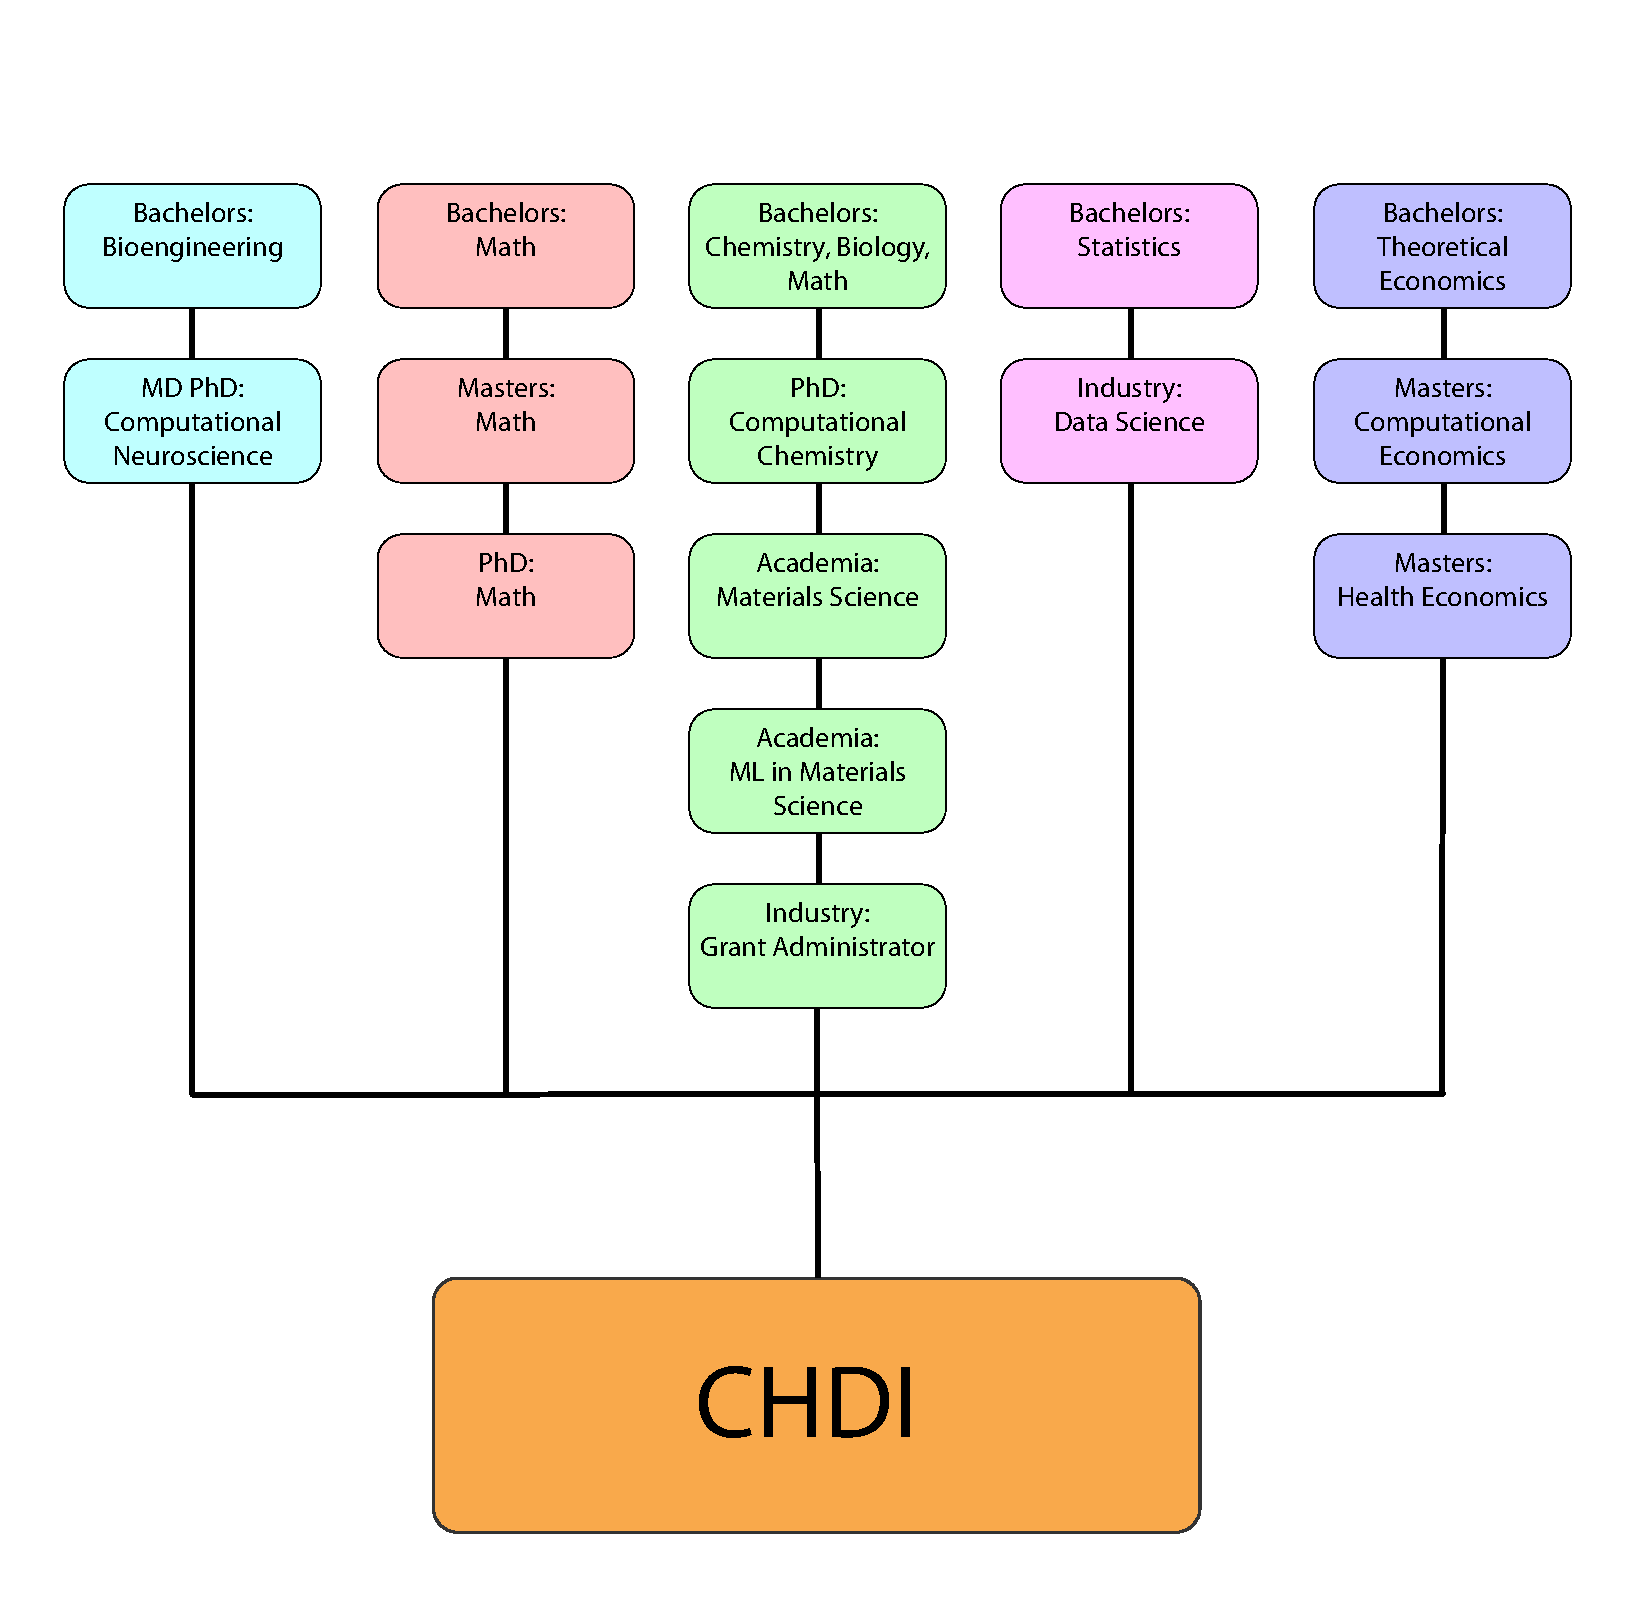
\includegraphics[width=1\columnwidth]{images/data_science_progression.pdf}	
		\end{column}
	\end{columns}
\end{frame}

\begin{frame}{What do we do?}
	\begin{itemize}
		\item PROOFcheck
			\begin{itemize}
					\item Department - Critical Care
					\item Respiratory failure prediction
					\item EMR based alerts
			\end{itemize}
		\item Metastatic Epidural Spinal Cord Compression
			\begin{itemize}
				\item Department - Radiation Oncology
				\item Early identification and remediation of spinal met progression
			\end{itemize}
		\item Outpatient Appointment Attendance 
			\begin{itemize}
				\item Department - Medicine
				\item Determine the probability of a patient not showing up to their appointment
				\item Optimize patient appointments
			\end{itemize}
	\end{itemize}
	
\end{frame}

\begin{frame}{Digital Transformation of Healthcare}
	\small
	\begin{itemize}
		\item What kind of questions can I answer using automatically collected data?
		\item What kind of data is collected by the hospital and how can I access the data?
		\item How much will it cost/save the hospital to implement the study as well as act on its results?
		\item What do I need to consider when designing a study using patient data? 
		\item How can I integrate automatic systems with collaborators to collect the desired data?
		\item How do I transform the data from its collected format to a format useful for analysis?
		\item How can I integrate the results of my study within the hospital system?
	\end{itemize}
\end{frame}


\begin{frame}{Case Study}
You have developed a new method of detecting sepsis in patients, which you think is better than the current sepsis criteria.
	\begin{itemize}
		\item How can you determine if your claim is true, retrospectively?
		
	\end{itemize}
\end{frame}


\begin{frame}{Bioinformatics Pipeline}
	\begin{center}
		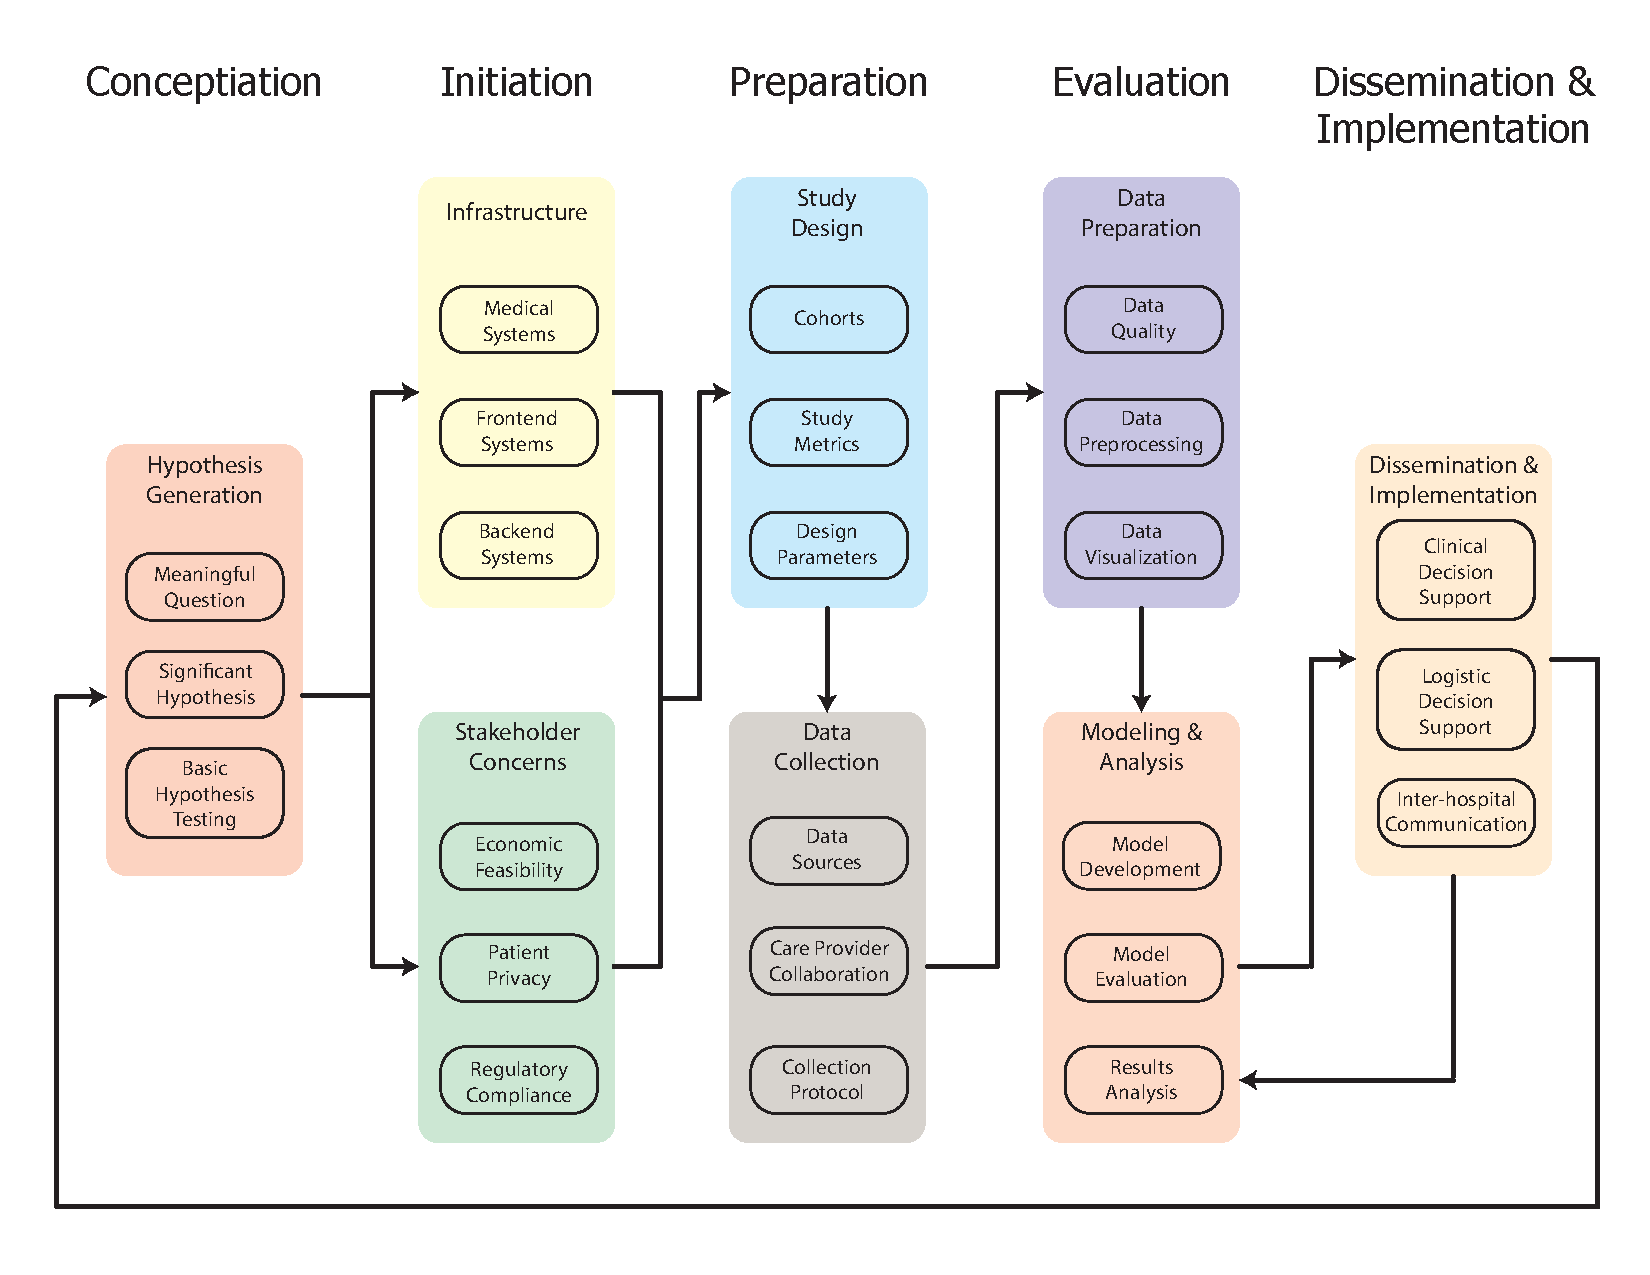
\includegraphics[width=0.8\textwidth]{images/informatics_pipeline.pdf}	
	\end{center}
\end{frame}


\begin{frame}{ETL \& Data Quality}
	\begin{center}
		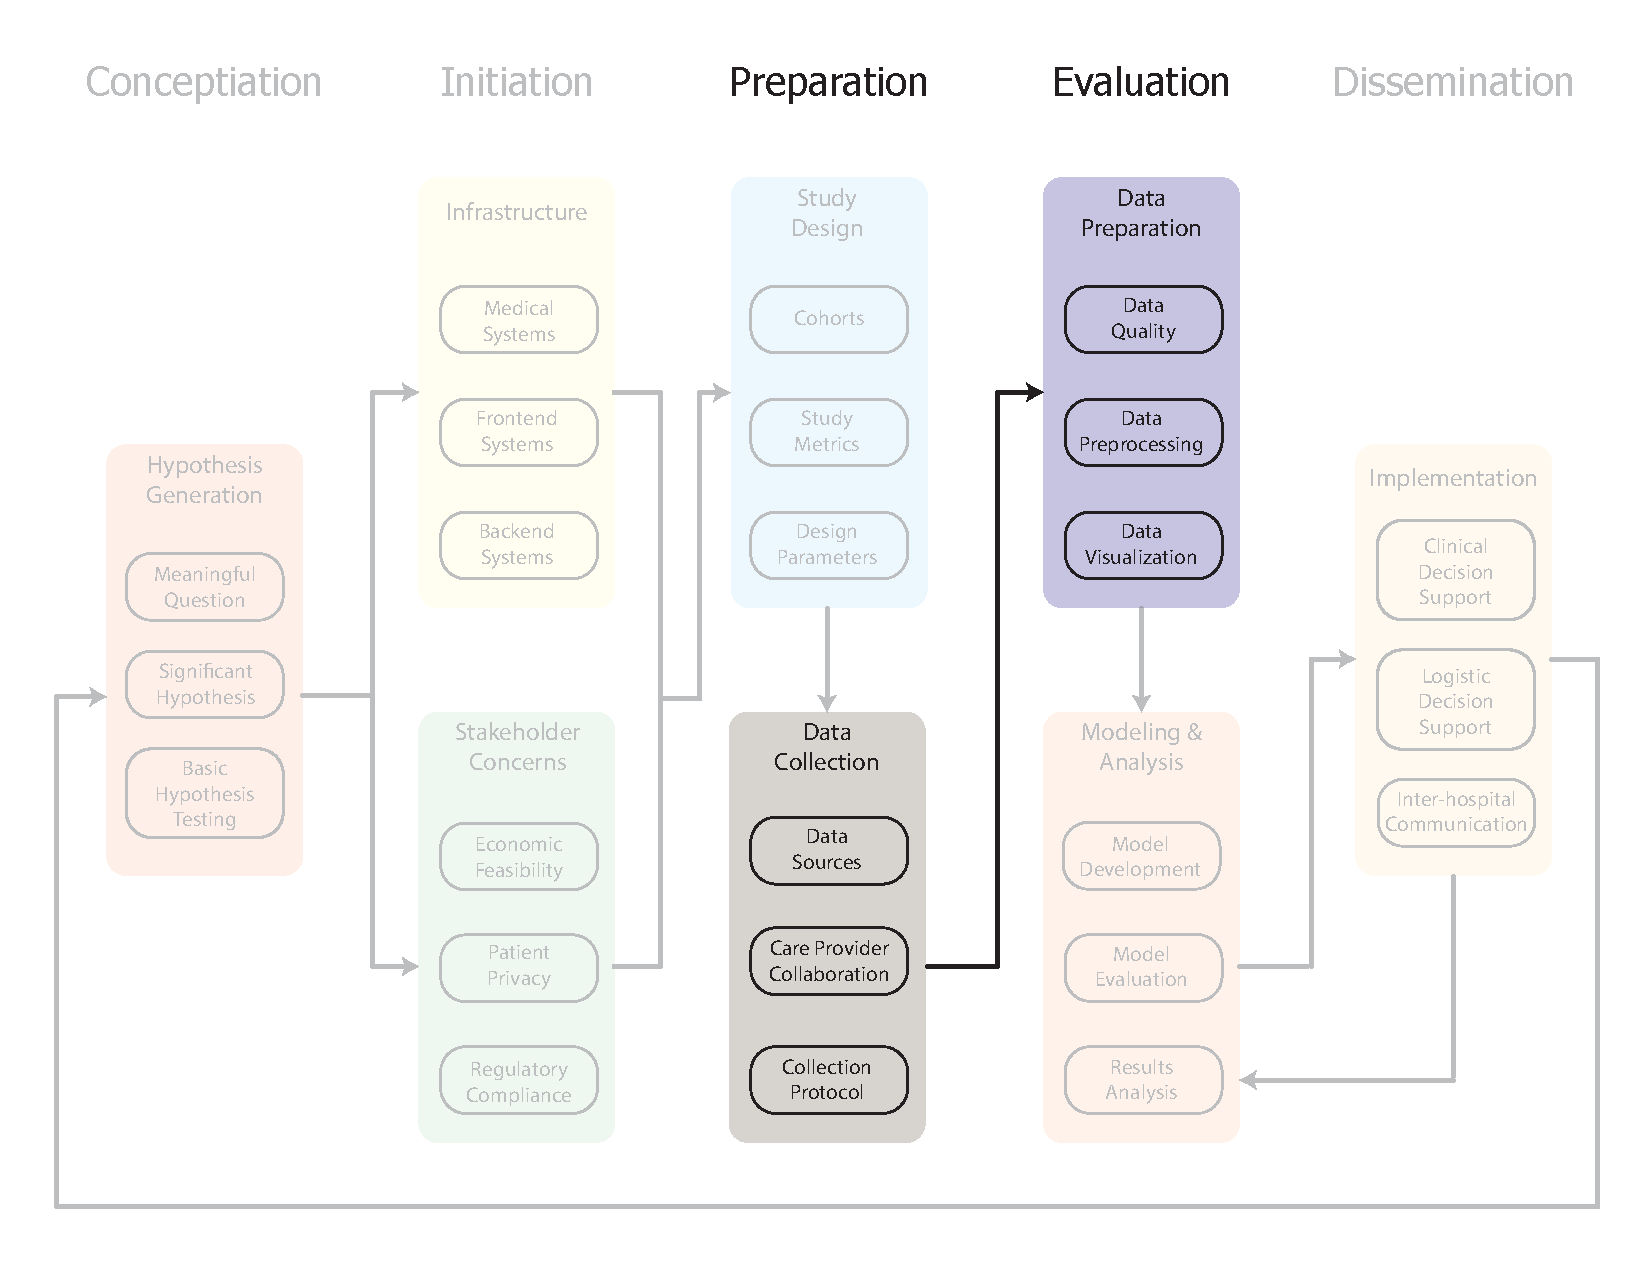
\includegraphics[width=0.8\textwidth]{images/informatics_pipeline_etl_data_quality.pdf}
	\end{center}
\end{frame}


\begin{frame}{Extract, Transform and Load (ETL)}
	\begin{center}
		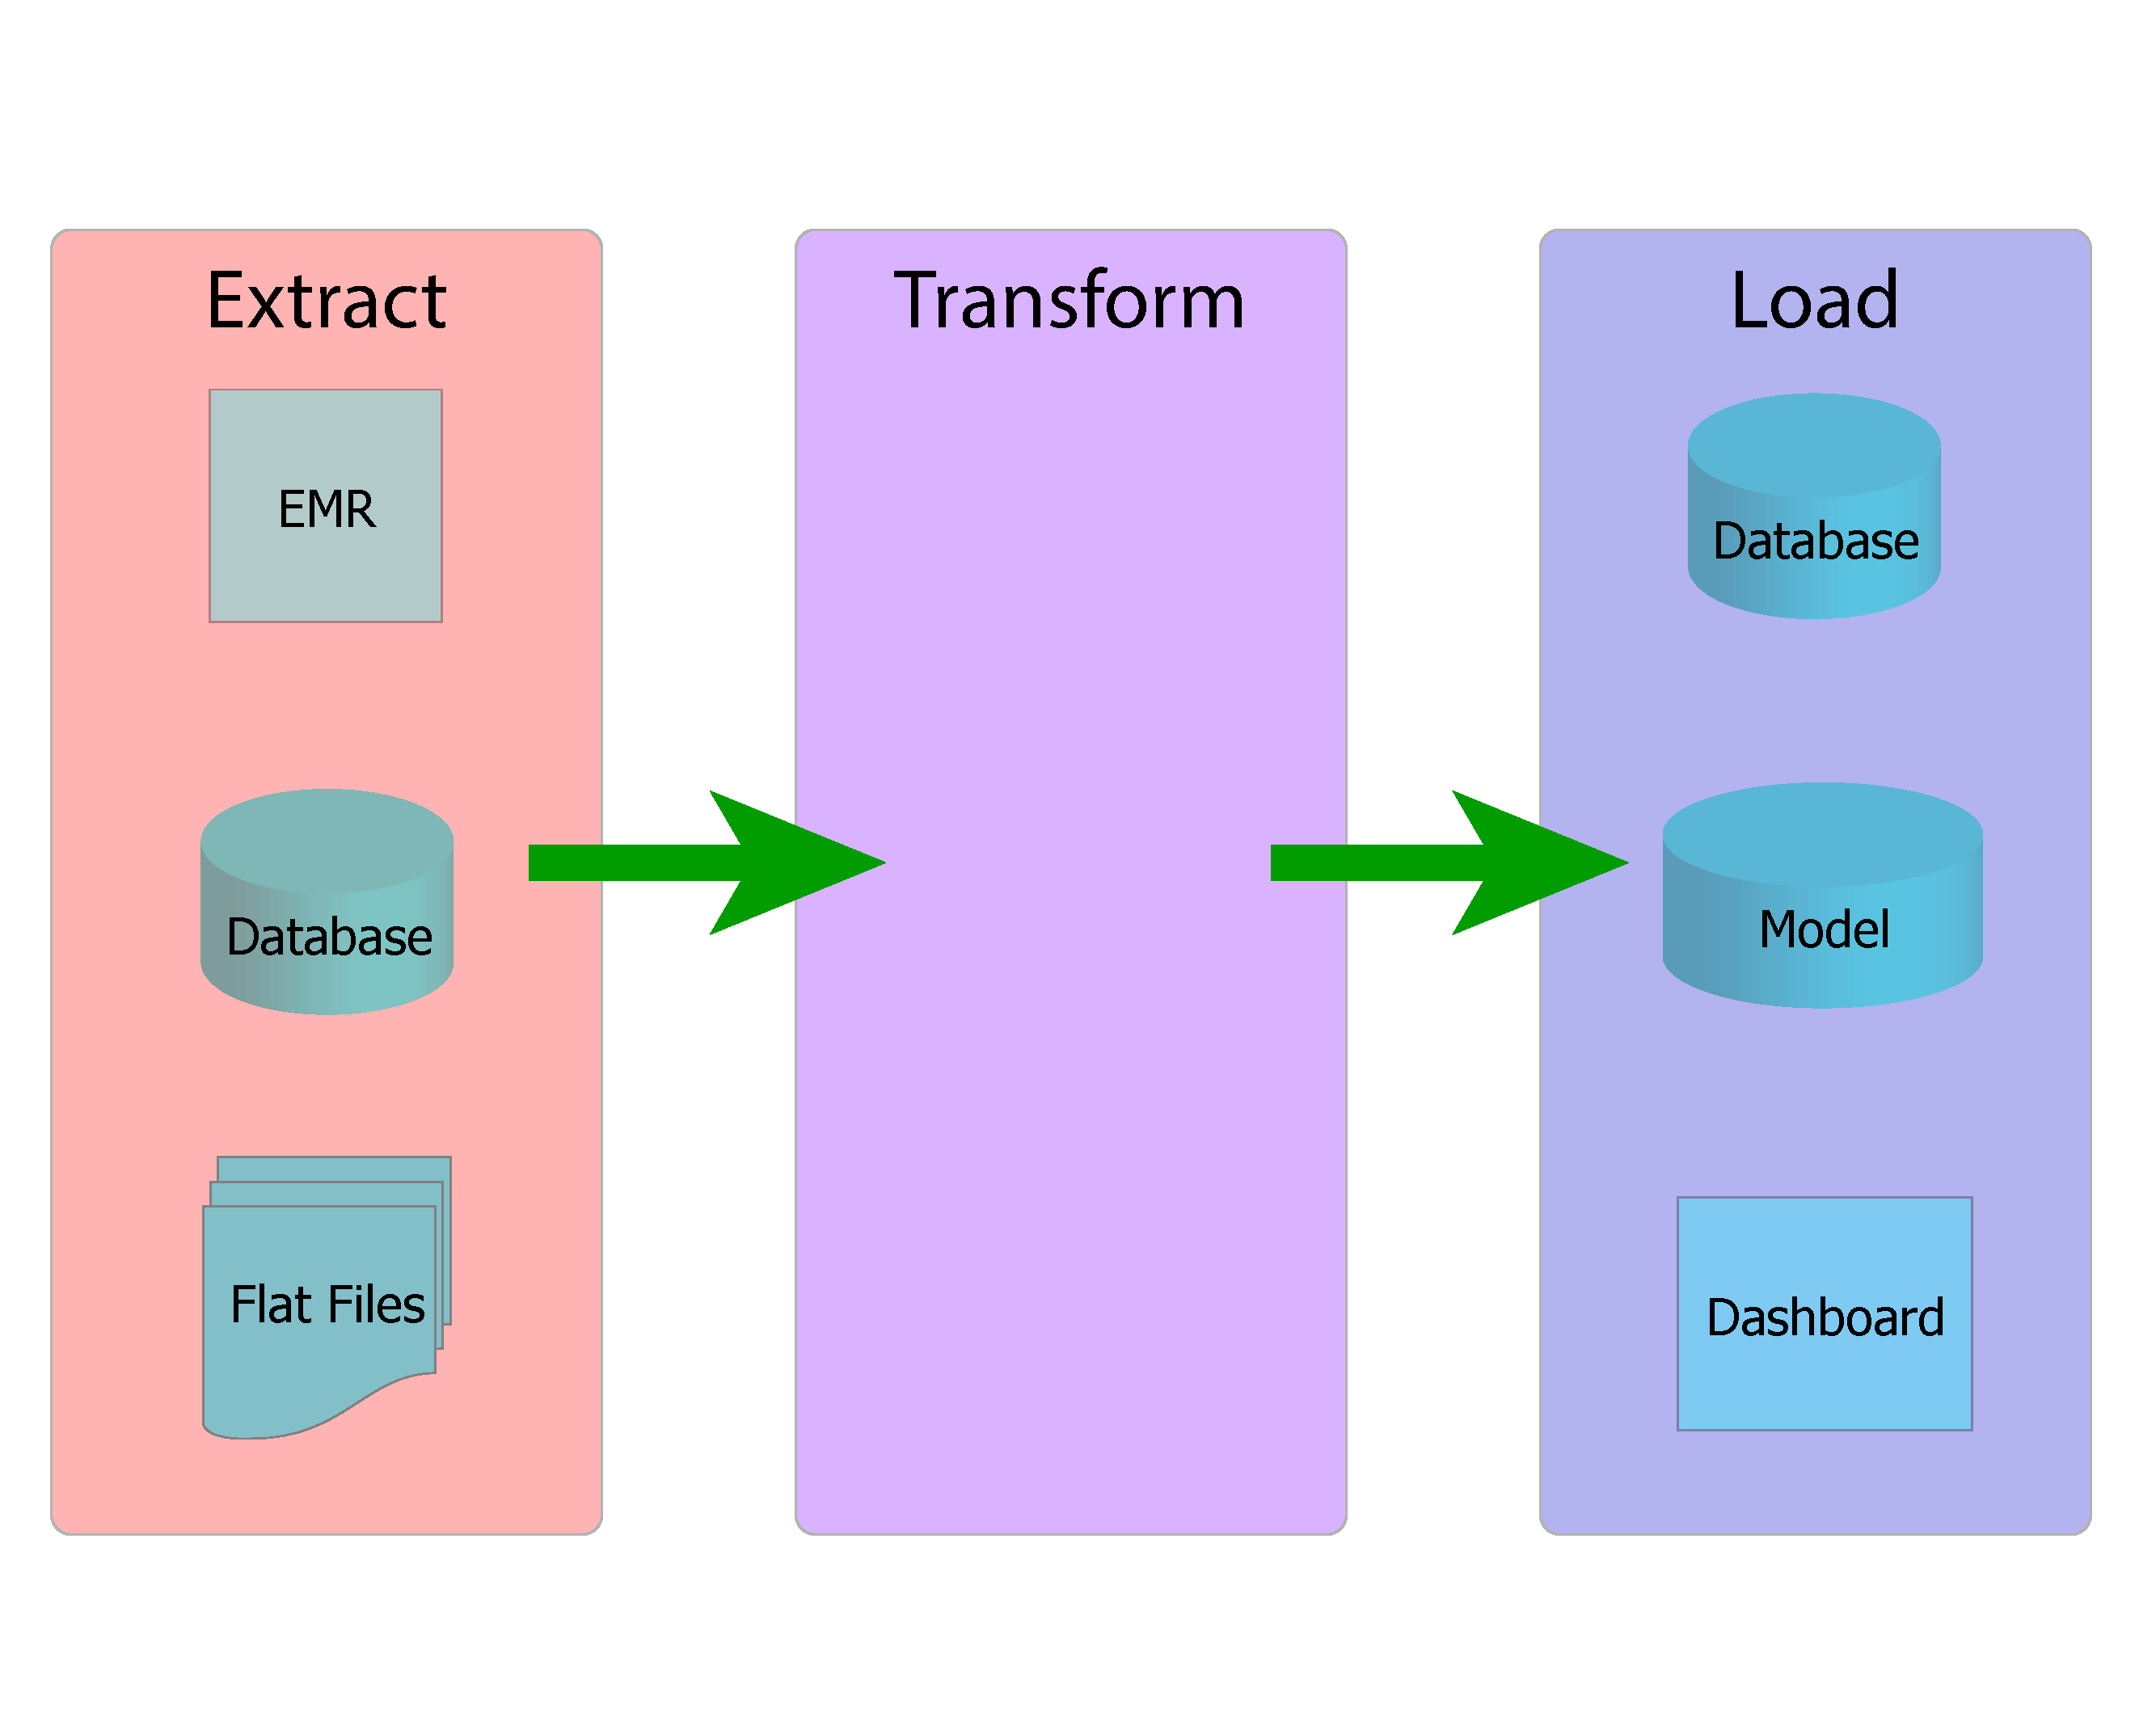
\includegraphics[width=0.75\textwidth]{images/etl_wo_transormations.pdf}
	\end{center}	
	\begin{itemize}
		\item What transformations would you want to do to your extracted data?
	\end{itemize}
\end{frame}


\begin{frame}{Extract, Transform and Load (ETL)}
	\begin{center}
		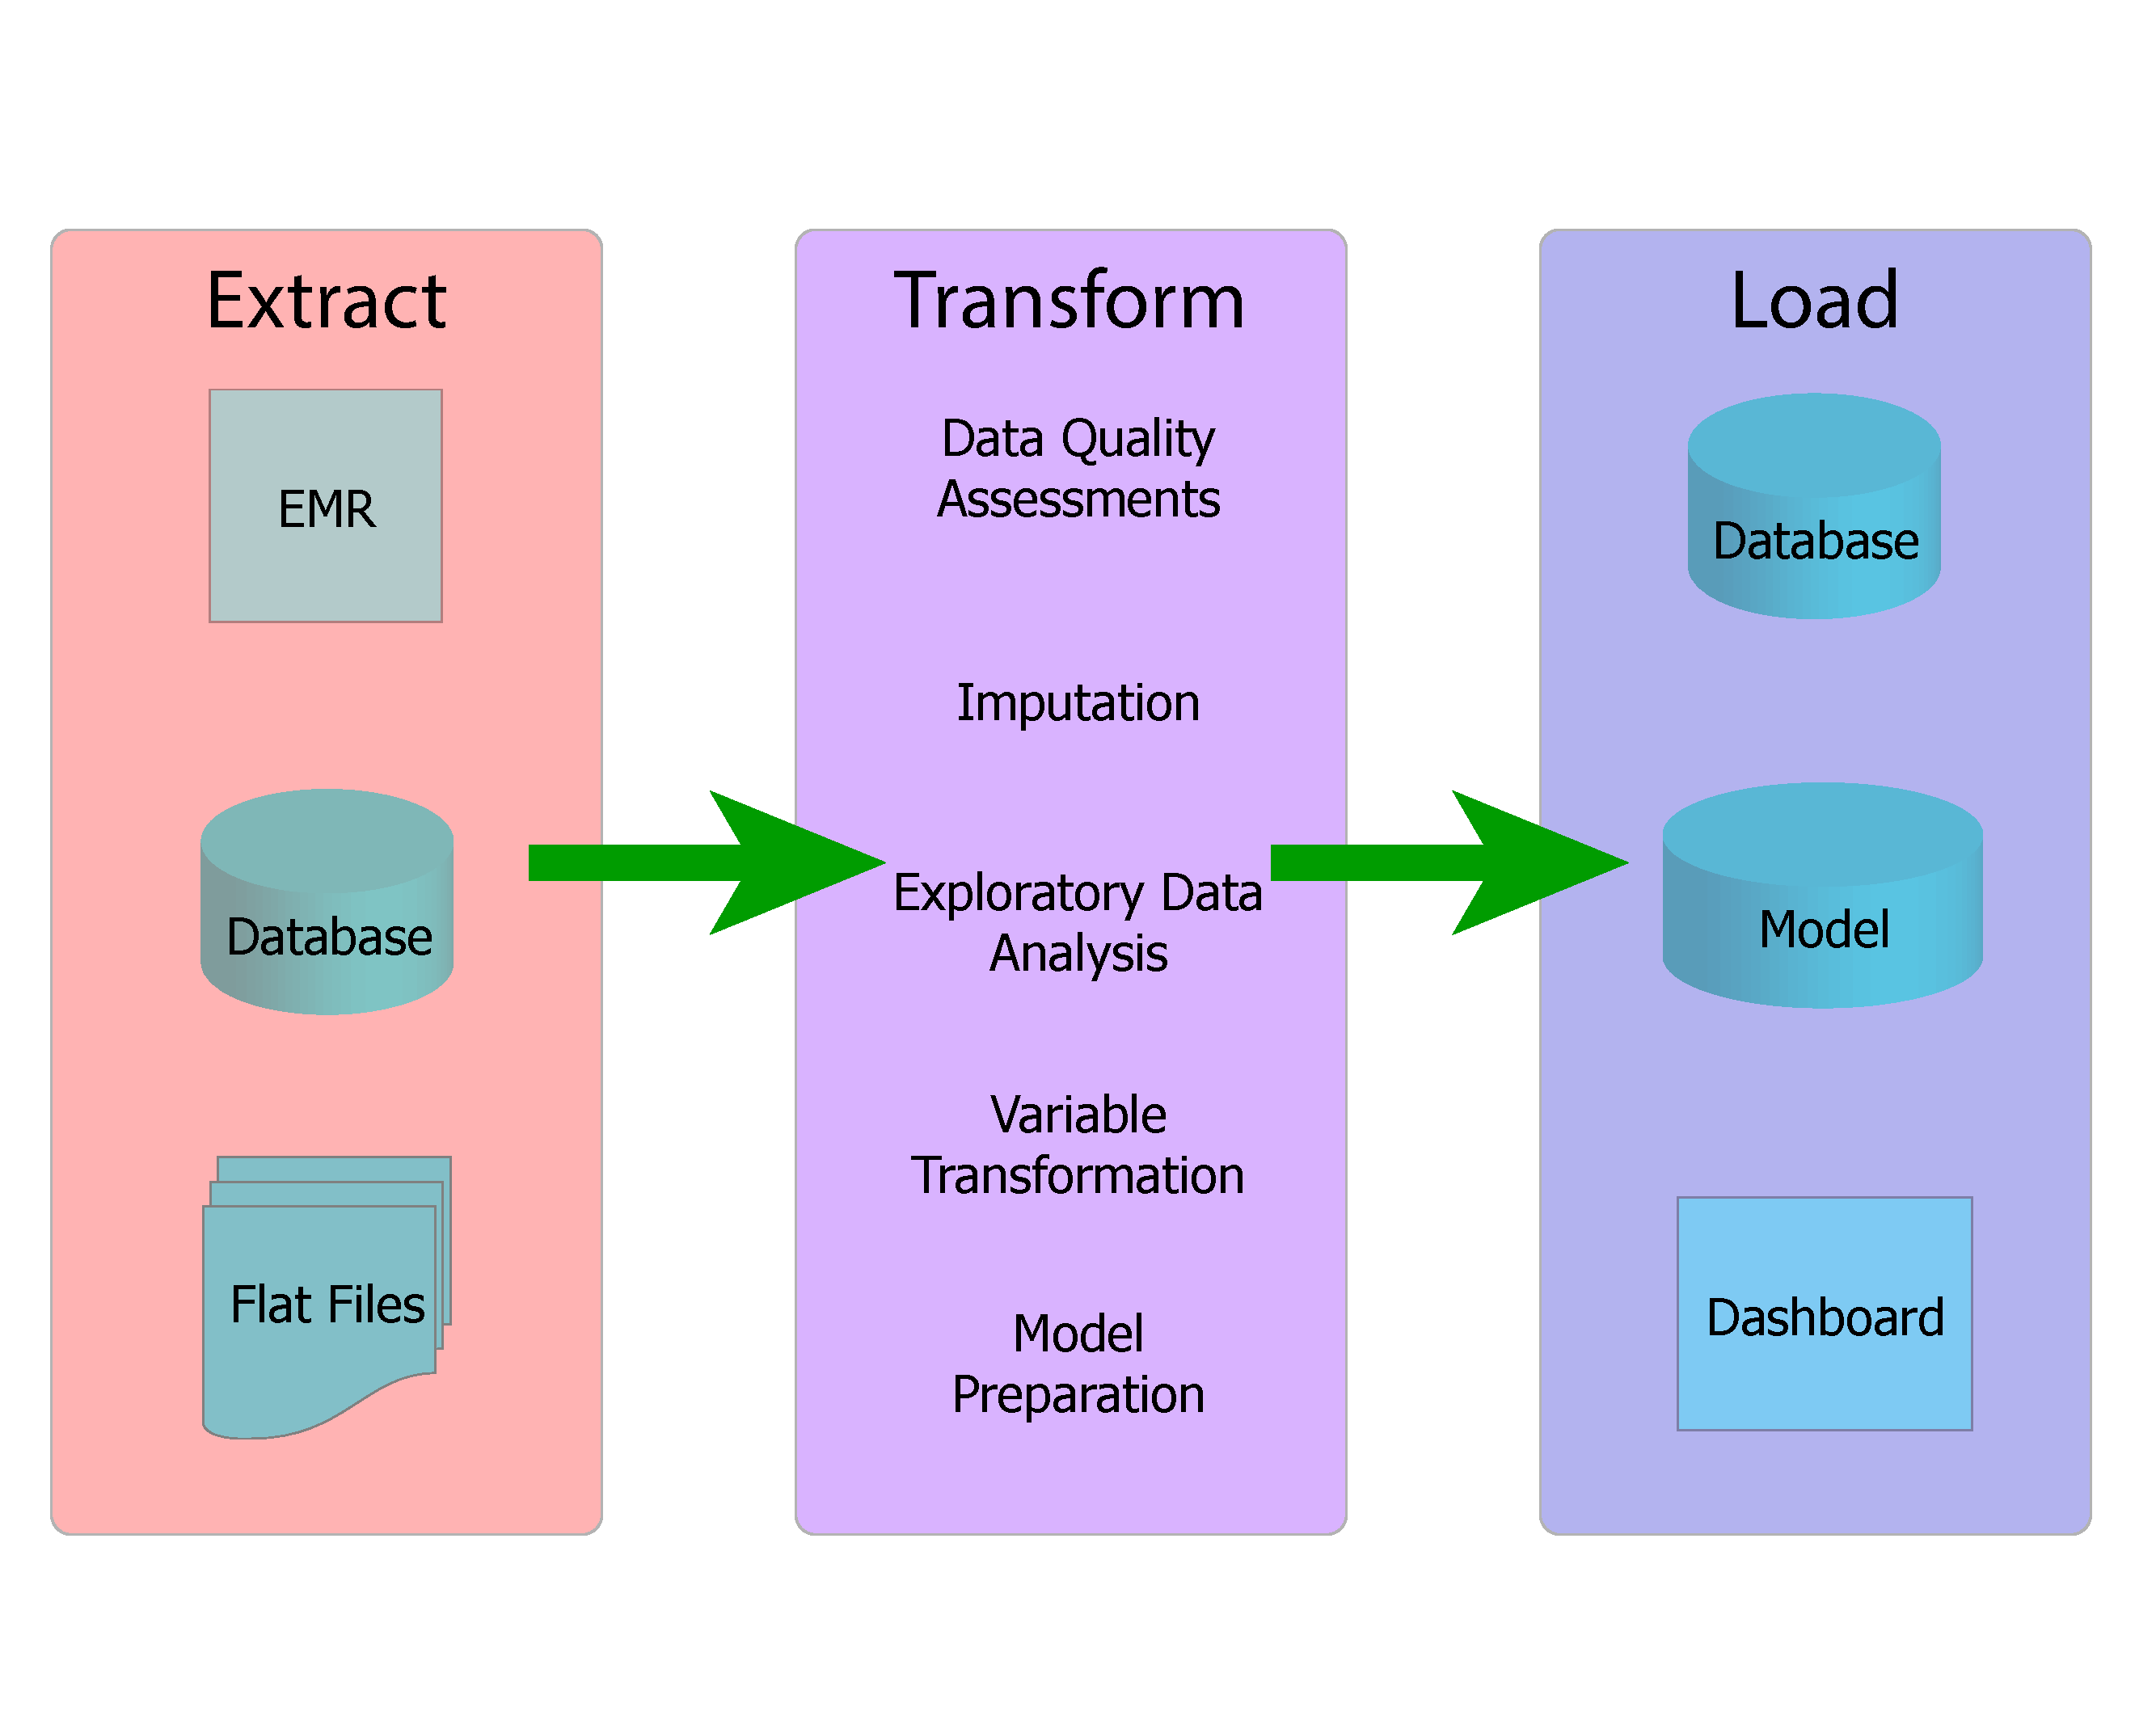
\includegraphics[width=0.9\textwidth]{images/etl.pdf}
	\end{center}	
\end{frame}



\note{
	\scriptsize
	\begin{itemize}
		\item Variable transformations
		\begin{itemize}
			\scriptsize
			\item Non-numerical to numerical data
			\item Extracting implied or hidden variables
			\item Connecting extraneous variables to current variables, e.g., weather to date
		\end{itemize}
		\item How can you convert non-numerical data to numerical data
		\begin{itemize}
			\scriptsize
			\item what kinds of non-numerical data are there - categorical (blood group, degree of Ab susceptibility/resistance), semi/unstructured (text, audio, video), boolean (test results), dates 
		\end{itemize}
		\item What makes a transformation useful? 
		\begin{itemize}
			\scriptsize
			\item What are all the different possible things you can extract from a date (season, days since equinox, hours since noon, is it happy hour, weekend)
			\item What other information can you connect to a date (weather, precipitation, barometric pressure, traffic accidents, sunrise, sunset, federal holiday, famous birthdays)			
		\end{itemize}
		
	\end{itemize}
}


\begin{frame}{Data Quality}
	\begin{center}
		Analysis is only ever as good as the data it's built upon.
	\end{center}
	\begin{itemize}%[<+(1)->]
		\item What is data quality? What makes data high quality vs low quality?
		\item Where along the process can you affect data quality?
		\item How can you design a study to collect high quality data (Quality assurance)?
		\item How can you identify and correct errors during and after data collection (Quality control)?
	\end{itemize}
\end{frame}

\note{
\scriptsize
	\begin{itemize}
		\item Data quality consists of the objective [accuracy, validity (not outside range of possibilities, all data is for the same pt, formatting requirements, DICOM dates), reliability (dx matches problem list matches coding), legibility (units, shorthand)] and subjective [completeness]
		\item Steps	
		\begin{itemize}
			\scriptsize
			\item Definition/Design - lack of clear definitions for data items/collection, incompatible units, precision, scope, depth
			\item Collection - not enough documentation (drug given/dosage altered but no start and end date), non-adherence to data definitions (collecting data outside of protocol time), human variance/error (bp cuff, RR, incorrect units), Orders are placed (procedures, medications) which are not connected to a rationale or sufficient reason 
			\item Processing - interpretation ('initial' lab, diagnosis date), coding error (mis-entering information such as order of birthdate, or height as 9 cm instead of 90 cm), random (mistyping, illegible handwriting), software errors, Assigning codes to problems treated vs problems tested and ruled out, which complaints do you code/document (doctors as coders)  
		\end{itemize} 
	\end{itemize}

}

\note{
	\scriptsize
	\begin{itemize}
		\item quality assurance - training of personnel (mock exams and reporting), site visits, reduce open-ended questions
		\item quality control - data monitoring (compare to independent source), hand verification, entering data in twice (by different sources), consistency checks
	\end{itemize}
}

%\begin{frame}{Data Collection and Ambiguity}
%	\begin{itemize}
%		\item Diagnosis Date
%		\item Medication Instructions
%		\begin{itemize}
%			\scriptsize
%			\item heparin flush (porcine) in NS Kit 100 unit/mL 500 UNITS. IV QDAY \#30 MILLILITERS
%			\item Heparin Lock Soln 100 unit/mL 500 UNITS. IV BID \#300 MILLILITERS refill x3 flush after each infusion
%			\item Heparin Sodium (Porcine) Syringe 10,000 unit/mL 18000 UNITs SC Q8HR \#180 MLs refill x5
%			\item heparin lock flush (porcine) syrg 100 unit/mL 100 UNITS. IV 3/wk 100 HS PRN \#200 MILLILITERS refi...
%			\item heparin (porcine) in 0.9\% NaCl IV Soln 100 unit/100 mL (1 unit/mL) 1-5 UNITS. IV QDAY \#100 MILLIL...
%		\end{itemize}
%	\end{itemize}
%\end{frame}




%\note{
%\scriptsize
%
%}

\begin{frame}{Quality Assurance - DICOM}
	\begin{itemize}
		\item DICOM - Digital Imaging and Communications in Medicine - is the international standard for medical images and related information. It defines the formats for medical images that can be exchanged with the data and quality necessary for clinical use
		\item DICOM groups information into data sets, e.g., an x-ray would contain the patient ID within the file, so that the image can never be separated from this information by mistake.
		\item \href{http://dicom.nema.org/medical/dicom/current/output/chtml/part05/sect_6.2.html\#table_6.2-1}{\color{blue}DICOM Value Representations}
	\end{itemize}
	
	\scriptsize{https://www.dicomstandard.org/about/}
\end{frame}

\begin{frame}{Quality Assurance - DICOM}
\scriptsize
\begin{tabular}{lll}
\toprule
                        name &  VR &                                              value \\
\midrule
                Group Length &  UL &                                                532 \\
                  Image Type &  CS &                                            DERIVED \\
               SOP Class UID &  UI &                          1.2.840.10008.5.1.4.1.1.2 \\
            SOP Instance UID &  UI &          1.2.840.114356.2008.11.30.12.34.2.329.999 \\
                  Study Date &  DA &                                           20081230 \\
                Content Date &  DA &                                           20081230 \\
                  Study Time &  TM &                                             122731 \\
                Content Time &  TM &                                         12299.0000 \\
                    Modality &  CS &                                                 CT \\
            Institution Name &  LO &                       Manhasset Diagnostic Imaging \\
                Station Name &  SH &                                                    \\
           Study Description &  LO &                  MOSES CT Outside Reference Images \\
     Procedure Code Sequence &  SQ &  [\{(0008, 0100): (0008, 0100) Code Value       ... \\
                  Code Value &  SH &                                      MOSESOUTREFCT \\
    Coding Scheme Designator &  SH &                                              GEIIS \\
       Coding Scheme Version &  SH &                                                  0 \\
                Code Meaning &  LO &                  MOSES CT Outside Reference Images \\
          Series Description &  LO &                                        Reformatted \\
    Referenced SOP Class UID &  UI &   1.2.840.113619.2.51762891606.1649.1005918257.250 \\
 Referenced SOP Instance UID &  UI &         1.2.840.114356.2008.11.30.12.34.2.329.1301 \\
\bottomrule
\end{tabular}
\end{frame}


\begin{frame}{Quality Assurance - DICOM}
\begin{center}
\begin{tabular}{lll}
\toprule
                        name &  VR &                                              value \\
\midrule
                  Study Date &  DA &                                           20081230 \\
                Content Date &  DA &                                           20081230 \\
                  Study Time &  TM &                                             122731 \\
                Content Time &  TM &                                         12299.0000 \\
\bottomrule
\end{tabular}
\end{center}
	\begin{itemize}
		\item \textbf{DA} - A string of characters of the format YYYYMMDD
		\item \textbf{TM} - A string of characters of the format HHMMSS.FFFFFF.  
		\begin{itemize}
			\item One or more of the components MM, SS, or FFFFFF may be unspecified as long as every component to the right of an unspecified component is also unspecified
		\end{itemize}		 
	\end{itemize}

	\begin{center}
		\large{Whose fault is this?}
	\end{center}
\end{frame}

\begin{frame}{Quality Control - Sepsis Case Study}
	My Sepsis metric depend on the following parameters
	\begin{itemize}
		\item Temperature
		\item Respiratory Rate
		\item BP
		\item HR
	\end{itemize}	
	\begin{center}
		How can I find the temperatures recorded from every patient in the hospital?
	\end{center}
\end{frame}


\begin{frame}
	\huge 
	\begin{center}
		To the SQL
	\end{center}
\end{frame}

\note{
	\begin{itemize}
		\scriptsize
		\item Explore the tables. go to findings.  Explain the lookup tables. Export Results
		\item determine the findingtypeid's you want to use from the table lookupfinding \\
			SELECT * \\
			FROM edm.lookupfinding \\
			WHERE LOWER(FINDINGDESC) like '\%temp\%'; 
		\item Determine which lab id you want from the most probable options \\
			SELECT nativefinding, numericfinding, findingtypeid, numericfindinglow, numericfindinghigh \\
			FROM edm.findings \\
			WHERE findingtypeid in (642, 806, 120,121, 134, 135); \\
		\item count the distinct MRNs \\
			SELECT COUNT(DISTINCT MRN) \\
			FROM  edm.findings \\
			WHERE findingtypeid = 121; \\
		\item select the data using the id you want \\
			SELECT nativefinding, numericfinding, findingtypeid, numericfindinglow, numericfindinghigh \\
			FROM  edm.findings \\
			WHERE findingtypeid = 121; \\
				 		
	\end{itemize}
}

\begin{frame}
	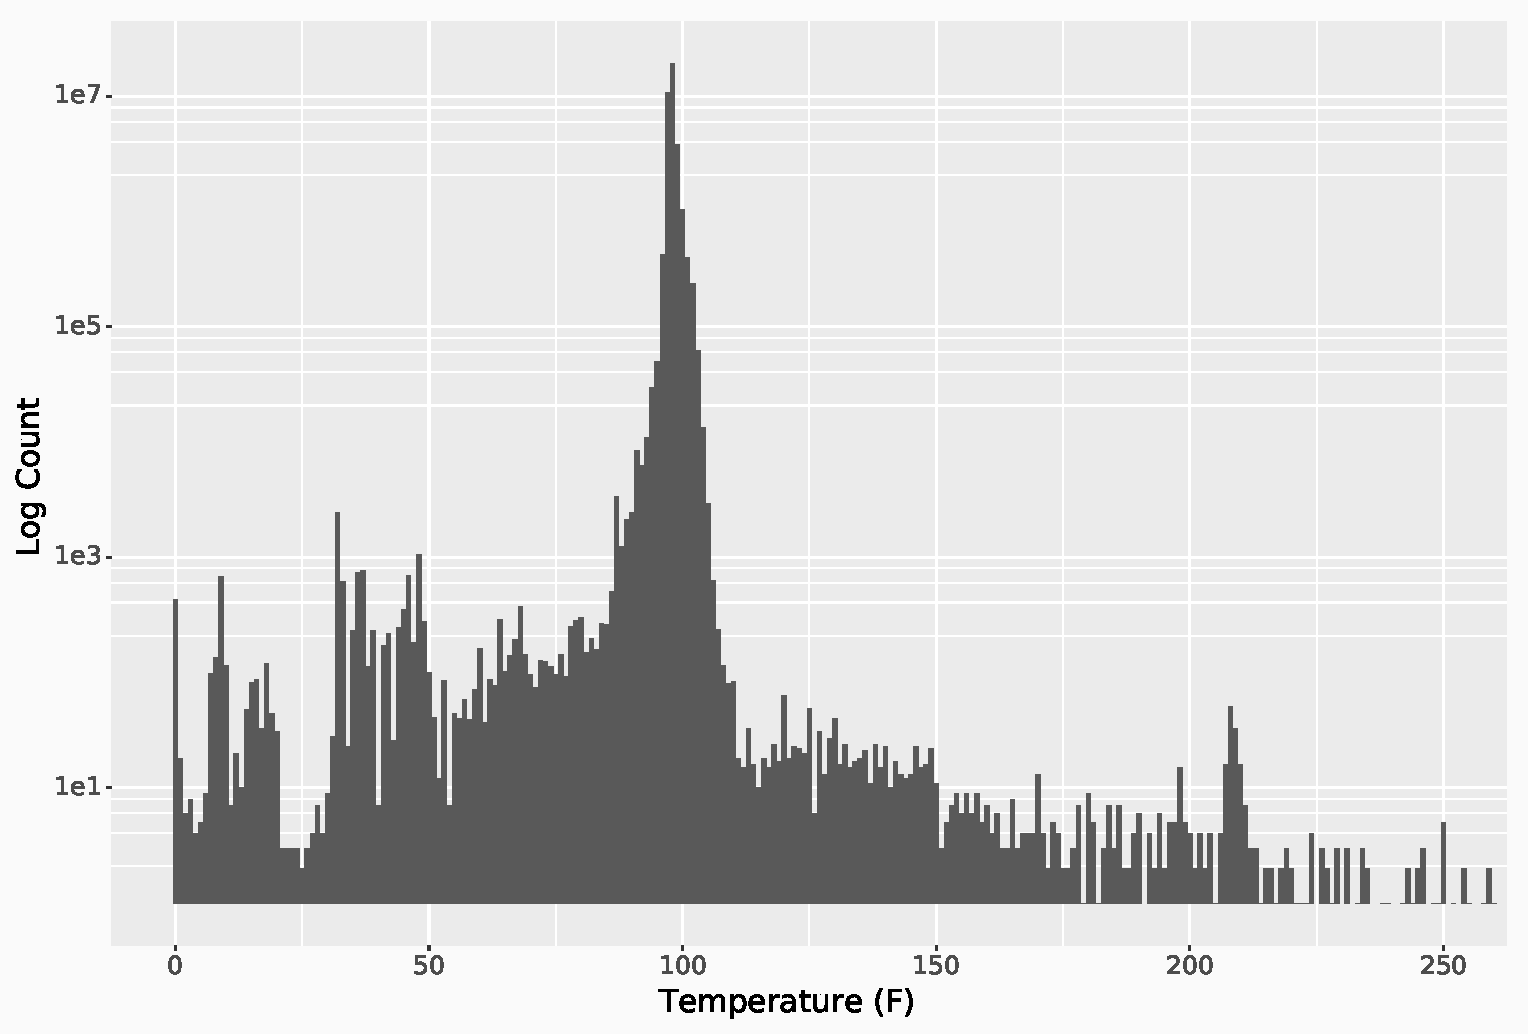
\includegraphics[width=\textwidth]{images/temp_value_counts.pdf}
\end{frame}

\note{
	\begin{itemize}
		\scriptsize
		\item How do you interpret the temps around 0 (probably had to enter something), how about around 37F (centigrade), how about 212, how about 95 (MICE)
		\item Let's take a look at an individual patient's data, who had a temp of 0
		\item maybe the data is being pulled from 5 different hospitals and it's the ETL which is causing the errors, because it doesn't know Celsius from F
		\item let's pick a patient whose temperature is zero and see what the rest of their temperature values look like (and then look at her results for that date)
	\end{itemize}
}

\begin{frame}
	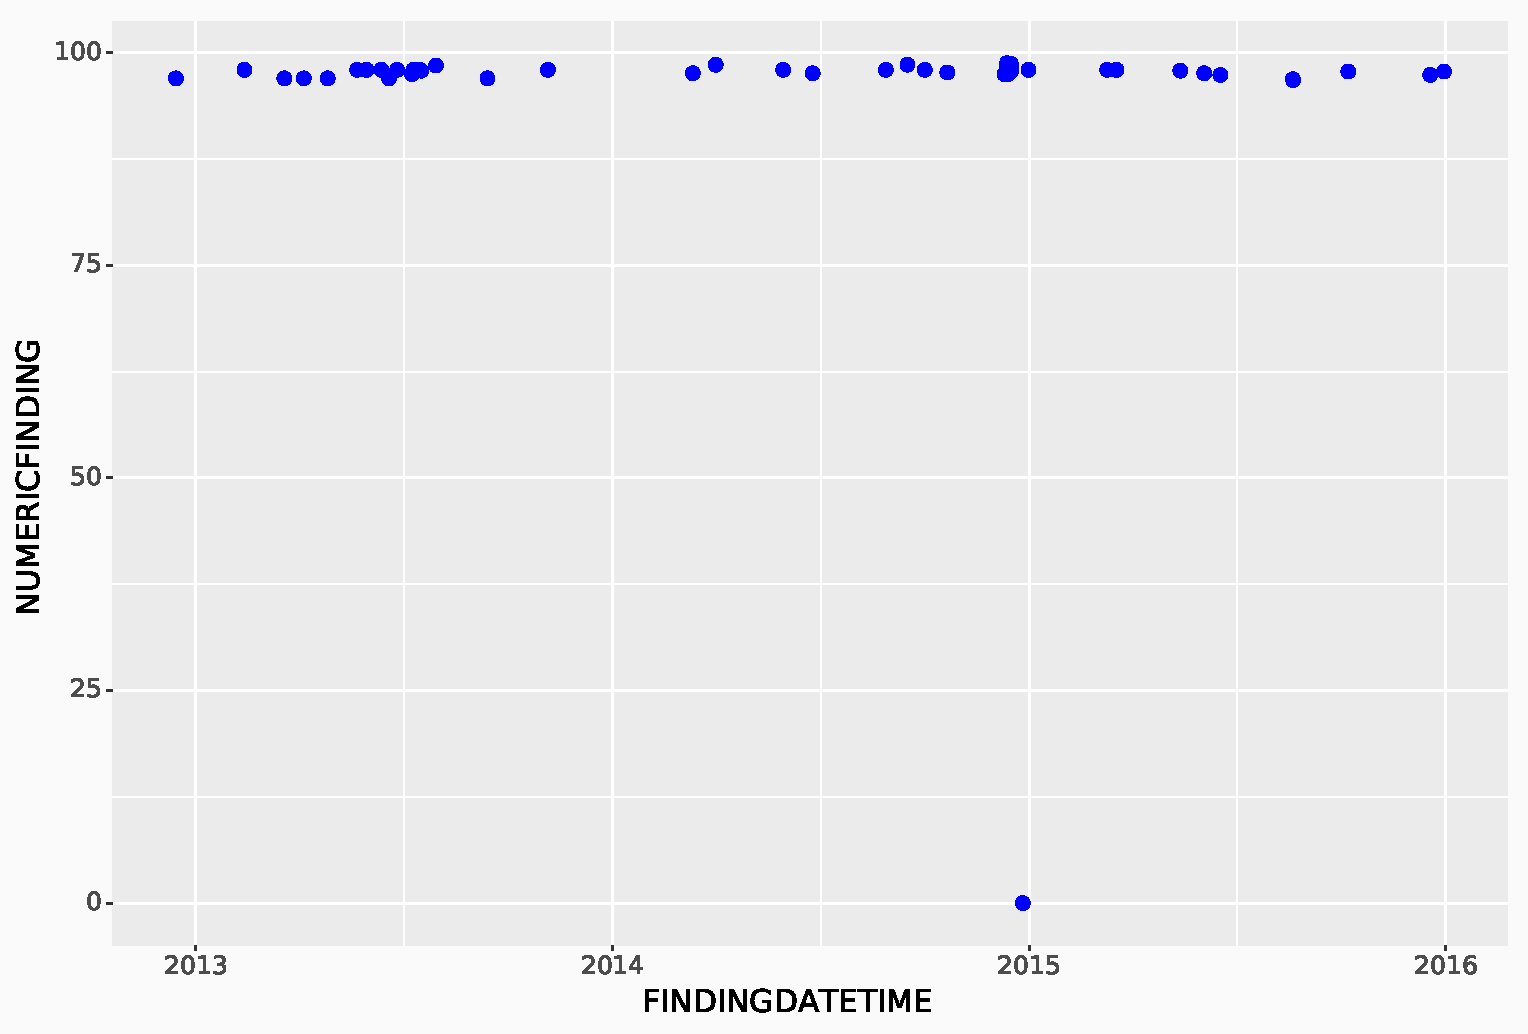
\includegraphics[width=\textwidth]{images/pt_temp_values.pdf}
\end{frame}


\begin{frame}{Associated Values}
\small
\begin{tabular}{llr}
\toprule
FINDINGDATETIME &               FINDINGDESC &  NUMERICFINDING \\
\midrule
     2014-12-26 &            PULSE OXIMETRY &           97.00 \\
     2014-12-26 &     WEIGHT/SCALE (ounces) &         2800.16 \\
     2014-12-26 &           HEIGHT (inches) &           62.00 \\
     2014-12-26 &  Diastolic Blood Pressure &           82.00 \\
     2014-12-26 &   Systolic Blood Pressure &          139.00 \\
     2014-12-26 &               HEIGHT (CM) &          157.48 \\
     2014-12-26 &                     PULSE &           75.00 \\
     2014-12-26 &           BODY MASS INDEX &           32.13 \\
     2014-12-26 &                   O2 SAT\% &           97.00 \\
     2014-12-26 &           TEMPERATURE (F) &            0.00 \\
     2014-12-26 &   Systolic Blood Pressure &          139.00 \\
     2014-12-26 &               WEIGHT (KG) &           79.38 \\
     2014-12-26 &  Diastolic Blood Pressure &           82.00 \\
\bottomrule
\end{tabular}
\end{frame}



\begin{frame}{Imputation and Extrapolation}
	\begin{center}
		\Large Can we develop a systematic way to deal with missing data
	\end{center}
	\begin{itemize}
		\item What are the different ways that data could be missing
	\end{itemize}
\end{frame}

\note{
	\scriptsize
	\begin{itemize}
		\item data could be MCAR, MAR, MNAR or because we are slicing the data into chunks smaller than the sampling rate
		\item Missing Data Procedure
		\begin{itemize}
			\scriptsize
			\item \textbf{Variable correctness} -  
var correctly derived/appropriate to include, e.g., complete or near-complete missingness or same value in all rows.
			\item \textbf{Time freq} - Ensure that time blocks used in time series data are appropriate to the task
			\item Determine how frequently every variable is measured
			\item Use the frequency range from the previous step for each variable to do ffill
			\item Encounters without data or good data cannot add value and should be dropped.
			\item Drop beginning blocks if empty, drop end blocks if dead or discharged
			\item \textbf{Imputation} - MICE, NN.  Cases where imputation should not be done are when the missingness itself is significant or if the imputation cannot be done by adding another class.  An example of the latter is would be if an x-ray is performed. X-rays not being performed are another class that can be added to the column.
			\item  Anything which is not imputed is masked (-9999, not 0)
		\end{itemize}
	\end{itemize}
}

\begin{frame}{Sources}
	\begin{itemize}
		\item \href{http://www.globalhealthworkforce.org/resources/who_improving_data_quality.pdf}{WHO data quality}
		\item \href{https://pdfs.semanticscholar.org/f68b/1f61568a15791dbc6f308ba73d39836fb47e.pdf}{Healthcare Data Warehousing and Quality Assurance}
		\item (2002). Defining and improving data quality in medical registries JAMIA, 9(6), 600-611.
	\end{itemize}

\end{frame}


\begin{frame}
	\begin{center}
 		{\Huge Thank You}
 		
 		\vspace{2cm}
 		
 		\href{https://github.com/MichoelSnow/crtp}{\color{blue}https://github.com/MichoelSnow/crtp}
 		
 		\vspace{1.5cm}
 		
 		msnow1@montefiore.org
	\end{center}

\end{frame}

\end{document}